\documentclass[12pt,a4paper]{article}
\usepackage[utf8]{inputenc}
\usepackage[T1]{fontenc}
\usepackage[brazil]{babel}
\usepackage{geometry}
\usepackage{amsmath}
\usepackage{amssymb}
\usepackage{tikz}
\usepackage{pgfplots}
\usepackage{booktabs}
\usepackage{array}
\usepackage{colortbl}
\usepackage{xcolor}
\usepackage{enumitem}
\usepackage{fancyhdr}
\usepackage{titlesec}
\usepackage{mdframed}
\usepackage{caption}
\usepackage{graphicx}
\usepackage{placeins}
\usepackage{listings}

% --- Configuração para o Código Python (Exercício 11) ---
\lstset{
    language=Python,
    basicstyle=\ttfamily\small,
    keywordstyle=\color{blue}\bfseries,
    stringstyle=\color{red},
    commentstyle=\color{green!50!black}\itshape,
    showstringspaces=false,
    frame=single,
    breaklines=true,
    numbers=left,
    numberstyle=\tiny\color{gray},
    backgroundcolor=\color{gray!5}
}

\pgfplotsset{compat=1.18}
\usetikzlibrary{arrows.meta, positioning, decorations.pathreplacing, calc}

\geometry{top=2.5cm, bottom=2.5cm, left=3cm, right=2.5cm}

\pagestyle{fancy}
\fancyhf{}
\rhead{Comunicação de Dados -- 1º semestre 2026}
\lhead{UTFPR -- Campus Apucarana}
\rfoot{\thepage}

\titleformat{\section}[block]{\large\bfseries}{}{0em}{}[{\titlerule[0.5pt]}]

\definecolor{destaque}{RGB}{0,70,140}
\definecolor{cinza}{RGB}{240,240,240}

\begin{document}

\begin{center}
    {\large\bfseries Universidade Tecnológica Federal do Paraná -- Campus Apucarana}\\[4pt]
    {\large Comunicação de Dados -- Trabalho -- 1º semestre}\\[2pt]
    {\large\itshape ``Trabalho sobre segunda parte do conteúdo''}\\[4pt]
    {\normalsize Prof.\ Dr.\ Luiz Fernando Carvalho}\\[6pt]
    \hrule
    \vspace{6pt}
    {\normalsize \textbf{Integrantes:} Elder Nunes Gonçalves \quad|\quad Felipe \quad|\quad Daniel Kroda}\\[4pt]
    \hrule
\end{center}

\vspace{1em}

% ============================================================
\section*{Exercício 1 \hfill \normalfont\small[1,0 ponto]}
% ============================================================

\subsection*{a) Portadoras}

\textbf{Sim, existem duas portadoras.}

Analisando a Figura 1, observam-se dois espectros de banda passante centrados em regiões distintas do espectro audível da linha telefônica (300--3400 Hz). A frequência fundamental de cada portadora é o ponto central de cada espectro:

\begin{itemize}
    \item \textbf{Portadora 1:} centrada em $f_{c1} = \dfrac{1070 + 1270}{2} = \mathbf{1170\,Hz}$
    \item \textbf{Portadora 2:} centrada em $f_{c2} = \dfrac{2025 + 2225}{2} = \mathbf{2125\,Hz}$
\end{itemize}

Cada portadora é modulada para representar sinais em uma direção de transmissão diferente, dentro da faixa utilizável da linha telefônica.

\subsection*{b) Modo de transmissão}

O modo de transmissão é \textbf{full-duplex}.

A figura mostra dois espectros distintos utilizados \textit{simultaneamente}: um para transmissão em uma direção (1070--1270 Hz) e outro para a direção oposta (2025--2225 Hz). Como ambas as direções operam ao mesmo tempo, sem necessidade de alternância, caracteriza-se o modo full-duplex. Isso é possível pela separação em frequência (FDM), que permite que os dois fluxos coexistam no mesmo meio físico sem interferência.

\subsection*{c) Multiplexação}

\textbf{Sim, ocorre multiplexação} -- especificamente \textbf{Multiplexação por Divisão de Frequência (FDM, \textit{Frequency Division Multiplexing})}.

O canal físico (linha telefônica, 300--3400 Hz) é dividido em duas sub-bandas que abrigam simultaneamente os dois sinais transmitidos em sentidos opostos. Cada sinal ocupa uma faixa de frequência distinta e exclusiva, caracterizando a divisão do meio entre múltiplos fluxos -- definição de multiplexação. Não há colisão entre os sinais porque operam em frequências diferentes.

\vspace{1em}

% ============================================================
\section*{Exercício 2 \hfill \normalfont\small[1,0 ponto]}
% ============================================================

\subsection*{Dados do problema}

O texto de 8 caracteres ``Aprovado'' é dividido em palavras de 2~bytes (16~bits).
Usando a tabela ASCII, cada caractere é representado por um valor hexadecimal:

\begin{center}
\begin{tabular}{|c|c|c|c|c|c|c|c|}
\hline
\rowcolor{destaque!30}
\textbf{A} & \textbf{p} & \textbf{r} & \textbf{o} &
\textbf{v} & \textbf{a} & \textbf{d} & \textbf{o} \\
\hline
\texttt{41} & \texttt{70} & \texttt{72} & \texttt{6F} &
\texttt{76} & \texttt{61} & \texttt{64} & \texttt{6F} \\
\hline
\end{tabular}
\end{center}

\noindent Agrupando em palavras de 16~bits (2 bytes por palavra):

\begin{center}
\begin{tabular}{cll}
\toprule
\textbf{Palavra} & \textbf{Hex} & \textbf{Binário (16 bits)} \\
\midrule
$W_1$ (A, p) & \texttt{4170} & \texttt{0100 0001 0111 0000} \\
$W_2$ (r, o) & \texttt{726F} & \texttt{0111 0010 0110 1111} \\
$W_3$ (v, a) & \texttt{7661} & \texttt{0111 0110 0110 0001} \\
$W_4$ (d, o) & \texttt{646F} & \texttt{0110 0100 0110 1111} \\
\bottomrule
\end{tabular}
\end{center}

\subsection*{Cálculo no Emissor}

O checksum é calculado pela soma em complemento de 1 de todas as palavras, seguida da inversão do resultado (complemento de 1 do total).

\subsubsection*{Passo 1 -- Soma $W_1 + W_2$}

\begin{center}
\begin{tabular}{r@{\hspace{0.5em}}l}
  & \texttt{0100 0001 0111 0000} \quad ($\mathtt{4170}_{16} = 16752_{10}$) \\
$+$ & \texttt{0111 0010 0110 1111} \quad ($\mathtt{726F}_{16} = 29295_{10}$) \\
\hline
  & \texttt{1011 0011 1101 1111} \quad ($\mathtt{B3DF}_{16} = 46047_{10}$) \\
\end{tabular}
\end{center}

\noindent Sem overflow (resultado $\leq$ \texttt{FFFF}).

\subsubsection*{Passo 2 -- Soma com $W_3$}

\begin{center}
\begin{tabular}{r@{\hspace{0.5em}}l}
  & \texttt{1011 0011 1101 1111} \quad ($\mathtt{B3DF}_{16}$) \\
$+$ & \texttt{0111 0110 0110 0001} \quad ($\mathtt{7661}_{16} = 30305_{10}$) \\
\hline
\textit{carry:} & \\
  & \texttt{1 0010 1010 0100 0000} \quad (overflow!) \\
\end{tabular}
\end{center}

\noindent Há overflow (bit 17 = 1). O carry é somado ao resultado (wrap-around):
\[
\mathtt{0010\,1010\,0100\,0000} + 1 = \mathtt{0010\,1010\,0100\,0001} = \mathtt{2A41}_{16}
\]

\subsubsection*{Passo 3 -- Soma com $W_4$}

\begin{center}
\begin{tabular}{r@{\hspace{0.5em}}l}
  & \texttt{0010 1010 0100 0001} \quad ($\mathtt{2A41}_{16}$) \\
$+$ & \texttt{0110 0100 0110 1111} \quad ($\mathtt{646F}_{16} = 25711_{10}$) \\
\hline
  & \texttt{1000 1110 1011 0000} \quad ($\mathtt{8EB0}_{16}$) \\
\end{tabular}
\end{center}

\noindent Sem overflow.

\subsubsection*{Passo 4 -- Complemento de 1 (inversão de todos os bits)}

\[
\text{Soma total} = \mathtt{8EB0}_{16}
= \mathtt{1000\,1110\,1011\,0000}_2
\]
\[
\boxed{\text{Checksum} = \overline{\mathtt{8EB0}}_{16}
= \mathtt{0111\,0001\,0100\,1111}_2 = \mathtt{714F}_{16}}
\]

\noindent O emissor transmite as quatro palavras seguidas do checksum:
\[
\underbrace{W_1,\, W_2,\, W_3,\, W_4}_{\text{dados}},\; \underbrace{\mathtt{714F}_{16}}_{\text{checksum}}
\]

\subsection*{Validação no Receptor}

O receptor soma todas as palavras recebidas, \textbf{incluindo o checksum}. Se o resultado for \texttt{FFFF}$_{16}$ (todos os bits em 1), a mensagem está íntegra.

\subsubsection*{Retomando: soma dos dados = \texttt{8EB0}$_{16}$}

\begin{center}
\begin{tabular}{r@{\hspace{0.5em}}l}
  & \texttt{1000 1110 1011 0000} \quad ($\mathtt{8EB0}_{16}$) \\
$+$ & \texttt{0111 0001 0100 1111} \quad ($\mathtt{714F}_{16}$ -- checksum) \\
\hline
  & \texttt{1111 1111 1111 1111} \quad ($\mathtt{FFFF}_{16}$) \\
\end{tabular}
\end{center}

\begin{mdframed}[backgroundcolor=green!10]
\textbf{Resultado:} A soma dá \texttt{FFFF}$_{16}$, confirmando que \textbf{não houve erros na transmissão}.
O receptor aceita a mensagem como válida.
\end{mdframed}

\vspace{1em}

% ============================================================
\section*{Exercício 3 \hfill \normalfont\small[1,0 ponto]}
% ============================================================

\subsection*{Identificação do algoritmo}

O algoritmo apresentado na Figura 2 é o \textbf{Go-Back-N com ARQ} (\textit{Automatic Repeat reQuest}).

As evidências são:
\begin{itemize}
    \item O emissor envia \textit{múltiplos frames} sem aguardar o ACK de cada um individualmente (janela de transmissão $> 1$);
    \item Quando o Frame 2 é perdido, o receptor descarta os frames subsequentes que chegam fora de ordem (Frame 3 é ignorado pelo receptor);
    \item Após detectar a falha (ausência de ACK do Frame 2), o emissor \textit{retransmite a partir do frame com erro} -- comportamento típico do Go-Back-N.
\end{itemize}

\subsection*{Descrição passo-a-passo da transmissão}

\begin{enumerate}[label=\textbf{Passo \arabic*.}, leftmargin=*, itemsep=4pt]
    \item \textbf{Envio do Frame 0:} O emissor A transmite o Frame 0 ao receptor B.

    \item \textbf{ACK 1 (confirmação do Frame 0):} O receptor B recebe o Frame 0 corretamente e envia o ACK 1, indicando que aguarda o próximo frame (Frame 1).

    \item \textbf{Envio do Frame 1:} Ainda dentro da janela de transmissão, o emissor envia o Frame 1 sem aguardar o ACK anterior (transmissão em pipeline).

    \item \textbf{ACK 2 (confirmação do Frame 1):} O receptor recebe o Frame 1 e envia ACK 2, aguardando agora o Frame 2.

    \item \textbf{Envio do Frame 2 -- perdido:} O emissor transmite o Frame 2, mas este é perdido no canal (indicado na figura como ``Perdido''). O receptor nunca o recebe.

    \item \textbf{Envio do Frame 3:} O emissor, sem saber da perda, continua e envia o Frame 3. O receptor B, porém, esperava o Frame 2 -- ao receber o Frame 3 fora de ordem, o \textbf{descarta} (no Go-Back-N o receptor não armazena frames fora de ordem).

    \item \textbf{Timeout / ausência de ACK 3:} O emissor percebe que não recebeu o ACK 3 dentro do tempo limite (timeout). Isso sinaliza que algo deu errado a partir do Frame 2.

    \item \textbf{Retransmissão a partir do Frame 2:} O emissor \textbf{retransmite o Frame 2} (e retransmite também quaisquer frames enviados após ele, como o Frame 3, caso necessário -- comportamento Go-Back-N).

    \item \textbf{ACK 4 (confirmação do Frame 2 retransmitido e do Frame 3):} O receptor recebe o Frame 2 retransmitido corretamente e, em seguida, o Frame 3 (também retransmitido). Confirma com o \textbf{ACK 4}, indicando que ambos foram recebidos e que aguarda agora o Frame 4.
\end{enumerate}

\vspace{1em}

% ============================================================
\section*{Exercício 4 \hfill \normalfont\small[1,0 ponto]}
% ============================================================

\subsection*{Resposta}

O \textbf{TDM Estatístico (STDM)} tende a ser \textbf{mais rápido} (maior eficiência de enlace) que o TDM Síncrono.

\subsection*{Justificativa}

\subsubsection*{TDM Síncrono}

No TDM Síncrono, o tempo do enlace é dividido em \textbf{slots fixos} e cada slot é atribuído a um canal de forma \textbf{determinística e periódica}, independentemente de o canal ter dados a enviar.

\begin{itemize}
    \item Se um canal estiver \textbf{ocioso} (sem dados a transmitir), seu slot é desperdiçado -- transmitido vazio.
    \item A capacidade total do enlace é distribuída igualmente entre todos os canais a todo momento.
    \item Exemplo: com 4 canais e 1 canal ocioso, 25\% da banda é desperdiçada em cada quadro.
\end{itemize}

\subsubsection*{TDM Estatístico (Assíncrono)}

No STDM, os slots \textbf{não são pré-atribuídos}. O multiplexador \textbf{aloca slots dinamicamente}, apenas para canais que possuem dados a transmitir.

\begin{itemize}
    \item Canais ociosos \textbf{não consomem} slots; sua capacidade é redistribuída entre os canais ativos.
    \item Cada frame carrega um \textbf{cabeçalho} (overhead) identificando a qual canal cada slot pertence -- isso é necessário porque a ordem não é mais fixa.
    \item A capacidade efetiva do enlace é aproveitada de forma \textbf{proporcional à demanda real} de cada canal.
\end{itemize}

\subsubsection*{Comparação resumida}

\begin{center}
\begin{tabular}{lcc}
\toprule
\textbf{Característica} & \textbf{TDM Síncrono} & \textbf{TDM Estatístico} \\
\midrule
Alocação de slots & Fixa & Dinâmica (por demanda) \\
Desperdício em canais ociosos & Sim & Não \\
Overhead de endereçamento & Não & Sim (pequeno) \\
Eficiência de enlace & Menor & \textbf{Maior} \\
Complexidade & Menor & Maior \\
Velocidade efetiva & Menor & \textbf{Maior} \\
\bottomrule
\end{tabular}
\end{center}

\begin{mdframed}[backgroundcolor=destaque!8]
\textbf{Conclusão:} O TDM Estatístico tende a ser mais rápido porque \textbf{elimina o desperdício de banda}
causado por slots vazios. Ao alocar capacidade somente quando há tráfego real, a taxa de transferência
útil sobre o mesmo enlace físico é maximizada. A desvantagem é a necessidade de overhead de identificação
por frame, mas esse custo é geralmente superado pelo ganho de eficiência.
\end{mdframed}

\vspace{1em}

% ============================================================
\section*{Exercício 5 \hfill \normalfont\small[1,0 ponto]}
% ============================================================

\subsection*{Análise das alternativas}

\begin{mdframed}[backgroundcolor=cinza, linewidth=0.5pt]
\textbf{Regra:} soma apenas as alternativas \textit{verdadeiras}.
\end{mdframed}

\vspace{0.5em}

\subsubsection*{Alternativa (1) -- \textcolor{green!50!black}{\textbf{VERDADEIRA}}}

\textit{``Stop-and-wait com ARQ é um caso particular do Go-Back-N com ARQ, em que o tamanho da janela de transmissão é 1.''}

\textbf{Correto.} No protocolo Go-Back-N, o emissor pode ter até $W$ frames não confirmados em trânsito simultaneamente. Quando $W = 1$, o emissor envia um frame e aguarda o ACK antes de enviar o próximo -- exatamente o comportamento do Stop-and-Wait. Portanto, Stop-and-Wait é de fato um caso especial de Go-Back-N com janela de tamanho 1.

\subsubsection*{Alternativa (2) -- \textcolor{red!70!black}{\textbf{FALSA}}}

\textit{``A largura de banda total mínima é de 540 kHz (5 canais $\times$ 100 kHz + 4 bandas de proteção $\times$ 10 kHz).''}

\textbf{Errado.} O cálculo correto é:
\[
    BW_{total} = 5 \times 100\,\text{kHz} + 4 \times 10\,\text{kHz} = 500 + 40 = \mathbf{540}\,\text{kHz}
\]

Aguarde -- o valor de 540 kHz \textit{está correto}. Entre 5 canais existem \textbf{4} bandas de proteção (entre canal 1--2, 2--3, 3--4 e 4--5). $540$ kHz é o valor correto.

\textbf{Revisando:} a alternativa 2 é \textcolor{green!50!black}{\textbf{VERDADEIRA}}.

\subsubsection*{Alternativa (4) -- \textcolor{green!50!black}{\textbf{VERDADEIRA}}}

\textit{``Na transmissão serial síncrona existe overhead.''}

\textbf{Correto.} Na transmissão síncrona, os dados são agrupados em \textit{frames} que contêm campos de controle: delimitadores de início/fim de frame (flags), endereços, campos de controle de sequência e campos de verificação de erros (FCS/CRC). Esses campos adicionais constituem o \textit{overhead} de protocolo -- informação extra além dos dados úteis.

\subsubsection*{Alternativa (8) -- \textcolor{red!70!black}{\textbf{FALSA}}}

\textit{``Considerando a ordem big-endian, o valor em decimal que representa o byte \texttt{10110011} é 205.''}

\textbf{Errado.} O byte \texttt{10110011} em binário, convertido para decimal é:
\[
    1\cdot2^7 + 0\cdot2^6 + 1\cdot2^5 + 1\cdot2^4 + 0\cdot2^3 + 0\cdot2^2 + 1\cdot2^1 + 1\cdot2^0
    = 128 + 32 + 16 + 2 + 1 = \mathbf{179}
\]
O valor correto é \textbf{179}, não 205. A ordem \textit{big-endian} se refere à ordenação de \textit{bytes} na memória (byte mais significativo primeiro), não à conversão de um único byte de binário para decimal -- portanto, não altera o resultado.

\subsubsection*{Alternativa (16) -- \textcolor{red!70!black}{\textbf{FALSA}}}

\textit{``Com números de sequência de 5 bits, os tamanhos máximos das janelas para Stop-and-Wait e Selective Repeat são, respectivamente, 31 e 16.''}

\textbf{Errado.} Com $n = 5$ bits de número de sequência, temos $2^5 = 32$ números de sequência possíveis (0 a 31). Os tamanhos máximos de janela são:

\begin{center}
\begin{tabular}{lll}
\toprule
\textbf{Protocolo} & \textbf{Tamanho máximo de janela} & \textbf{Valor (n=5)} \\
\midrule
Stop-and-Wait & $1$ & $1$ \\
Go-Back-N & $2^n - 1$ & $31$ \\
Selective Repeat & $2^{n-1}$ & $16$ \\
\bottomrule
\end{tabular}
\end{center}

A alternativa confunde Go-Back-N (janela = 31) com Stop-and-Wait. Para Stop-and-Wait, a janela é sempre \textbf{1} independentemente do número de bits de sequência.

\subsubsection*{Alternativa (32) -- \textcolor{red!70!black}{\textbf{FALSA}}}

\textit{``A distância de Hamming mínima no CRC equivale à quantidade de bits do código gerador menos um. Coloca-se essa distância mínima como preenchimento (padding) no cálculo do CRC.''}

\textbf{Errado em dois aspectos:}
\begin{itemize}
    \item A \textbf{distância de Hamming mínima} do CRC não é simplesmente ``bits do gerador menos um'' -- ela depende do polinômio gerador específico escolhido e do tamanho da mensagem;
    \item O \textbf{padding} (preenchimento com zeros) no CRC corresponde ao \textit{grau do polinômio gerador} (quantidade de bits do gerador menos 1), e é acrescentado ao \textit{final da mensagem} antes da divisão, não relacionado à distância de Hamming. A distância de Hamming mínima é uma propriedade de detecção de erros do código, não um parâmetro de cálculo inserido na mensagem.
\end{itemize}

\subsection*{Resultado}

As alternativas verdadeiras são: \textbf{(1), (2) e (4)}.

\[
\boxed{\text{Soma} = 1 + 2 + 4 = \mathbf{7}}
\]

\vspace{1em}

% ============================================================
\section*{Exercício 6 \hfill \normalfont\small[1,0 ponto]}
% ============================================================

\subsection*{Alternativa correta}

\begin{center}
\large\textbf{b) unipolar, RZ, NRZ, polar}
\end{center}

\subsection*{Análise de cada sinal}

\subsubsection*{Sinal (a) -- dados: 1\,0\,1\,1\,0}

O sinal apresenta:
\begin{itemize}
    \item Para o bit \textbf{1}: nível de tensão \textbf{positivo} durante todo o período do bit (sem retorno a zero).
    \item Para o bit \textbf{0}: nível \textbf{zero} durante todo o período do bit.
\end{itemize}
Usa apenas dois níveis: positivo e zero (nunca negativo).
$\Rightarrow$ \textbf{Unipolar NRZ} (Non-Return-to-Zero unipolar).

\subsubsection*{Sinal (b) -- dados: 0\,1\,0\,0\,1}

O sinal apresenta:
\begin{itemize}
    \item Para o bit \textbf{1}: o sinal vai ao nível positivo na \textbf{primeira metade} do período e \textbf{retorna a zero} na segunda metade.
    \item Para o bit \textbf{0}: permanece em zero.
\end{itemize}
Há retorno explícito ao nível zero dentro do período de cada bit.
$\Rightarrow$ \textbf{RZ} (Return-to-Zero).

\subsubsection*{Sinal (c) -- dados: 0\,1\,0\,0\,1}

O sinal apresenta:
\begin{itemize}
    \item Para o bit \textbf{1}: nível positivo durante \textbf{todo} o período.
    \item Para o bit \textbf{0}: nível negativo (ou zero) durante todo o período, \textbf{sem} retorno a zero no meio do bit.
\end{itemize}
Usa dois níveis fixos sem retorno ao zero: $\Rightarrow$ \textbf{NRZ}.

\subsubsection*{Sinal (d) -- dados: 0\,1\,0\,0\,1}

O sinal apresenta:
\begin{itemize}
    \item Usa \textbf{dois níveis de tensão} (positivo e negativo), porém com uma transição \textbf{no meio} do período de cada bit.
    \item Para o bit \textbf{1}: transição de positivo para negativo (ou vice-versa) no centro do bit.
    \item Para o bit \textbf{0}: sem transição no centro.
\end{itemize}
Característica de codificação \textbf{Polar} com transição diferencial.
$\Rightarrow$ \textbf{Polar} (ex.: Manchester diferencial ou NRZ-I).

\begin{mdframed}[backgroundcolor=yellow!15]
\textbf{Resposta final: alternativa b) \quad unipolar~|~RZ~|~NRZ~|~polar}
\end{mdframed}

\vspace{1em}

% ============================================================
\section*{Exercício 7 \hfill \normalfont\small[0,4 ponto]}
% ============================================================

\textbf{Método NRZ-L (\textit{Non-Return-to-Zero Level}):}
\begin{itemize}
    \item Bit \textbf{0} $\rightarrow$ nível de sinal \textbf{positivo} ($+V$)
    \item Bit \textbf{1} $\rightarrow$ nível de sinal \textbf{negativo} ($-V$)
\end{itemize}

O enunciado informa que o \textbf{último nível de sinal anterior foi positivo}.

\vspace{1em}

% --- a) 00000000 ---
\subsection*{a) Fluxo: \texttt{00000000}}

Todos os bits são 0, portanto o sinal permanece em nível positivo ($+V$) durante toda a sequência. Como já estava em $+V$ antes do início, não há transição.

\begin{center}
\begin{tikzpicture}[xscale=0.85, yscale=0.7]
    % Grid
    \draw[gray!30, very thin] (0,-1.5) grid (8.5,1.5);
    % Axes
    \draw[->] (-0.3,0) -- (8.8,0) node[right] {Tempo};
    \draw[->] (0,-1.7) -- (0,1.8) node[above] {Sinal};
    % Level labels
    \node[left, font=\small] at (0,1.2) {$+V$};
    \node[left, font=\small] at (0,-1.2) {$-V$};
    \draw[dashed, gray!50] (0,1.2) -- (8.5,1.2);
    \draw[dashed, gray!50] (0,-1.2) -- (8.5,-1.2);
    % Bit markers
    \foreach \i/\b in {0/0,1/0,2/0,3/0,4/0,5/0,6/0,7/0} {
        \node[above, font=\tiny, color=destaque] at (\i+0.5, 1.5) {\b};
        \draw[gray!40, thin] (\i,0.05) -- (\i,-0.05);
    }
    % Signal: all +V
    \draw[blue!70!black, very thick] (0,1.2) -- (8,1.2);
    % Vertical lines for bit boundaries
    \foreach \i in {1,2,3,4,5,6,7} {
        \draw[gray!40, thin, dashed] (\i,-1.3) -- (\i,1.3);
    }
    \node[below, font=\small] at (4,-1.8) {\texttt{00000000}: sinal constante em $+V$};
\end{tikzpicture}
\end{center}

\vspace{0.5em}

% --- b) 11111111 ---
\subsection*{b) Fluxo: \texttt{11111111}}

Todos os bits são 1, portanto o sinal permanece em nível negativo ($-V$) durante toda a sequência. Há uma transição de $+V$ para $-V$ no instante inicial (antes do primeiro bit).

\begin{center}
\begin{tikzpicture}[xscale=0.85, yscale=0.7]
    \draw[gray!30, very thin] (0,-1.5) grid (8.5,1.5);
    \draw[->] (-0.3,0) -- (8.8,0) node[right] {Tempo};
    \draw[->] (0,-1.7) -- (0,1.8) node[above] {Sinal};
    \node[left, font=\small] at (0,1.2) {$+V$};
    \node[left, font=\small] at (0,-1.2) {$-V$};
    \draw[dashed, gray!50] (0,1.2) -- (8.5,1.2);
    \draw[dashed, gray!50] (0,-1.2) -- (8.5,-1.2);
    \foreach \i/\b in {0/1,1/1,2/1,3/1,4/1,5/1,6/1,7/1} {
        \node[above, font=\tiny, color=destaque] at (\i+0.5, 1.5) {\b};
        \draw[gray!40, thin] (\i,0.05) -- (\i,-0.05);
    }
    % Signal: all -V (transition at 0)
    \draw[blue!70!black, very thick] (0,-1.2) -- (8,-1.2);
    \foreach \i in {1,2,3,4,5,6,7} {
        \draw[gray!40, thin, dashed] (\i,-1.3) -- (\i,1.3);
    }
    \node[below, font=\small] at (4,-1.8) {\texttt{11111111}: sinal constante em $-V$};
\end{tikzpicture}
\end{center}

\vspace{0.5em}

% --- c) 01010101 ---
\subsection*{c) Fluxo: \texttt{01010101}}

O sinal alterna entre $+V$ (bit 0) e $-V$ (bit 1) a cada bit. O sinal inicial começa em $+V$ (bit 0).

\begin{center}
\begin{tikzpicture}[xscale=0.85, yscale=0.7]
    \draw[gray!30, very thin] (0,-1.5) grid (8.5,1.5);
    \draw[->] (-0.3,0) -- (8.8,0) node[right] {Tempo};
    \draw[->] (0,-1.7) -- (0,1.8) node[above] {Sinal};
    \node[left, font=\small] at (0,1.2) {$+V$};
    \node[left, font=\small] at (0,-1.2) {$-V$};
    \draw[dashed, gray!50] (0,1.2) -- (8.5,1.2);
    \draw[dashed, gray!50] (0,-1.2) -- (8.5,-1.2);
    \foreach \i/\b in {0/0,1/1,2/0,3/1,4/0,5/1,6/0,7/1} {
        \node[above, font=\tiny, color=destaque] at (\i+0.5, 1.5) {\b};
    }
    % 01010101: +V -V +V -V +V -V +V -V
    % bit 0 (0): x=0..1, +V
    \draw[blue!70!black, very thick] (0,1.2) -- (1,1.2);
    \draw[blue!70!black, very thick] (1,1.2) -- (1,-1.2);
    % bit 1 (1): x=1..2, -V
    \draw[blue!70!black, very thick] (1,-1.2) -- (2,-1.2);
    \draw[blue!70!black, very thick] (2,-1.2) -- (2,1.2);
    % bit 2 (0): x=2..3, +V
    \draw[blue!70!black, very thick] (2,1.2) -- (3,1.2);
    \draw[blue!70!black, very thick] (3,1.2) -- (3,-1.2);
    % bit 3 (1): x=3..4, -V
    \draw[blue!70!black, very thick] (3,-1.2) -- (4,-1.2);
    \draw[blue!70!black, very thick] (4,-1.2) -- (4,1.2);
    % bit 4 (0): x=4..5, +V
    \draw[blue!70!black, very thick] (4,1.2) -- (5,1.2);
    \draw[blue!70!black, very thick] (5,1.2) -- (5,-1.2);
    % bit 5 (1): x=5..6, -V
    \draw[blue!70!black, very thick] (5,-1.2) -- (6,-1.2);
    \draw[blue!70!black, very thick] (6,-1.2) -- (6,1.2);
    % bit 6 (0): x=6..7, +V
    \draw[blue!70!black, very thick] (6,1.2) -- (7,1.2);
    \draw[blue!70!black, very thick] (7,1.2) -- (7,-1.2);
    % bit 7 (1): x=7..8, -V
    \draw[blue!70!black, very thick] (7,-1.2) -- (8,-1.2);
    \foreach \i in {1,2,3,4,5,6,7} {
        \draw[gray!40, thin, dashed] (\i,-1.3) -- (\i,1.3);
    }
    \node[below, font=\small] at (4,-1.8) {\texttt{01010101}: alternância máxima entre $+V$ e $-V$};
\end{tikzpicture}
\end{center}

\vspace{0.5em}

% --- d) 00110011 ---
\subsection*{d) Fluxo: \texttt{00110011}}

\begin{center}
\begin{tikzpicture}[xscale=0.85, yscale=0.7]
    \draw[gray!30, very thin] (0,-1.5) grid (8.5,1.5);
    \draw[->] (-0.3,0) -- (8.8,0) node[right] {Tempo};
    \draw[->] (0,-1.7) -- (0,1.8) node[above] {Sinal};
    \node[left, font=\small] at (0,1.2) {$+V$};
    \node[left, font=\small] at (0,-1.2) {$-V$};
    \draw[dashed, gray!50] (0,1.2) -- (8.5,1.2);
    \draw[dashed, gray!50] (0,-1.2) -- (8.5,-1.2);
    \foreach \i/\b in {0/0,1/0,2/1,3/1,4/0,5/0,6/1,7/1} {
        \node[above, font=\tiny, color=destaque] at (\i+0.5, 1.5) {\b};
    }
    % 00110011: +V +V -V -V +V +V -V -V
    % bits 0,1 (0,0): +V
    \draw[blue!70!black, very thick] (0,1.2) -- (2,1.2);
    \draw[blue!70!black, very thick] (2,1.2) -- (2,-1.2);
    % bits 2,3 (1,1): -V
    \draw[blue!70!black, very thick] (2,-1.2) -- (4,-1.2);
    \draw[blue!70!black, very thick] (4,-1.2) -- (4,1.2);
    % bits 4,5 (0,0): +V
    \draw[blue!70!black, very thick] (4,1.2) -- (6,1.2);
    \draw[blue!70!black, very thick] (6,1.2) -- (6,-1.2);
    % bits 6,7 (1,1): -V
    \draw[blue!70!black, very thick] (6,-1.2) -- (8,-1.2);
    \foreach \i in {1,2,3,4,5,6,7} {
        \draw[gray!40, thin, dashed] (\i,-1.3) -- (\i,1.3);
    }
    \node[below, font=\small] at (4,-1.8) {\texttt{00110011}: pares de bits idênticos alternando};
\end{tikzpicture}
\end{center}

\vspace{1em}

% ============================================================
\section*{Exercício 8 \hfill \normalfont\small[0,6 ponto]}
% ============================================================

\subsection*{Regra Manchester (IEEE 802.3)}

\begin{itemize}
    \item Bit \textbf{0} $\rightarrow$ transição de \textbf{$+V$ para $-V$} no meio do período (descida).
    \item Bit \textbf{1} $\rightarrow$ transição de \textbf{$-V$ para $+V$} no meio do período (subida).
    \item As transições no meio do bit são \textbf{obrigatórias} e servem também como sincronismo.
    \item Podem ocorrer transições adicionais entre bits consecutivos de mesmo tipo para garantir a transição obrigatória no centro.
\end{itemize}

%------- (a) 00000000 -------
\subsection*{a) Sequência: \texttt{00000000}}

Todos os bits são 0 $\Rightarrow$ cada bit: $+V$ na primeira metade $\to$ $-V$ na segunda metade.
Entre bits consecutivos iguais (0$\to$0), há transição de retorno ($-V \to +V$) na borda entre os bits.

\begin{figure}[!htbp]
\centering
\begin{tikzpicture}[scale=0.95]
  \def\high{0.8}
  \def\low{-0.8}
  \draw[->,thick] (-0.3,0) -- (8.8,0) node[right] {Tempo};
  \draw[->,thick] (0,\low-0.3) -- (0,\high+0.5) node[above] {Sinal};
  \node[left,font=\small] at (0,\high) {$+V$};
  \node[left,font=\small] at (0,\low)  {$-V$};
  \draw[dashed,gray!60] (-0.1,\high) -- (8.6,\high);
  \draw[dashed,gray!60] (-0.1,\low)  -- (8.6,\low);
  % Bit 0: first half +V, second half -V
  % Between 0->0: transition -V -> +V at bit boundary
  \foreach \i in {0,...,7}{
    % first half: +V
    \draw[blue,very thick] (\i,\high) -- (\i+0.5,\high);
    % middle transition: +V -> -V
    \draw[blue,very thick] (\i+0.5,\high) -- (\i+0.5,\low);
    % second half: -V
    \draw[blue,very thick] (\i+0.5,\low) -- (\i+1,\low);
    % boundary transition (return) for i>0: handled by next bit's first half
    \ifnum\i>0
      \draw[blue,very thick] (\i,\low) -- (\i,\high);
    \fi
    \draw (\i,0.07) -- (\i,-0.07);
    \node[below,font=\small\ttfamily] at (\i+0.5,-0.95) {0};
  }
  \draw (8,0.07) -- (8,-0.07);
\end{tikzpicture}
\caption{Manchester -- sequência \texttt{00000000}: transições obrigatórias no centro de cada bit (0 = descida)}
\end{figure}

%------- (b) 11111111 -------
\subsection*{b) Sequência: \texttt{11111111}}

Todos os bits são 1 $\Rightarrow$ cada bit: $-V$ na primeira metade $\to$ $+V$ na segunda metade.
Entre bits consecutivos iguais (1$\to$1), há transição de retorno ($+V \to -V$) na borda entre os bits.

\begin{figure}[!htbp]
\centering
\begin{tikzpicture}[scale=0.95]
  \def\high{0.8}
  \def\low{-0.8}
  \draw[->,thick] (-0.3,0) -- (8.8,0) node[right] {Tempo};
  \draw[->,thick] (0,\low-0.3) -- (0,\high+0.5) node[above] {Sinal};
  \node[left,font=\small] at (0,\high) {$+V$};
  \node[left,font=\small] at (0,\low)  {$-V$};
  \draw[dashed,gray!60] (-0.1,\high) -- (8.6,\high);
  \draw[dashed,gray!60] (-0.1,\low)  -- (8.6,\low);
  % Bit 1: first half -V, second half +V
  \foreach \i in {0,...,7}{
    \draw[blue,very thick] (\i,\low) -- (\i+0.5,\low);
    \draw[blue,very thick] (\i+0.5,\low) -- (\i+0.5,\high);
    \draw[blue,very thick] (\i+0.5,\high) -- (\i+1,\high);
    \ifnum\i>0
      \draw[blue,very thick] (\i,\high) -- (\i,\low);
    \fi
    \draw (\i,0.07) -- (\i,-0.07);
    \node[below,font=\small\ttfamily] at (\i+0.5,-0.95) {1};
  }
  \draw (8,0.07) -- (8,-0.07);
\end{tikzpicture}
\caption{Manchester -- sequência \texttt{11111111}: transições obrigatórias no centro de cada bit (1 = subida)}
\end{figure}

%------- (c) 01010101 -------
\subsection*{c) Sequência: \texttt{01010101}}

Bits alternados: entre bits diferentes não há transição na borda (a segunda metade de um bit já está no nível correto para a primeira metade do próximo).

\begin{figure}[!htbp]
\centering
\begin{tikzpicture}[scale=0.95]
  \def\high{0.8}
  \def\low{-0.8}
  \draw[->,thick] (-0.3,0) -- (8.8,0) node[right] {Tempo};
  \draw[->,thick] (0,\low-0.3) -- (0,\high+0.5) node[above] {Sinal};
  \node[left,font=\small] at (0,\high) {$+V$};
  \node[left,font=\small] at (0,\low)  {$-V$};
  \draw[dashed,gray!60] (-0.1,\high) -- (8.6,\high);
  \draw[dashed,gray!60] (-0.1,\low)  -- (8.6,\low);
  \def\bits{{0,1,0,1,0,1,0,1}}
  \foreach \i in {0,...,7}{
    \pgfmathtruncatemacro{\bit}{\bits[\i]}
    \ifnum\bit=0
      \draw[blue,very thick] (\i,\high) -- (\i+0.5,\high);
      \draw[blue,very thick] (\i+0.5,\high) -- (\i+0.5,\low);
      \draw[blue,very thick] (\i+0.5,\low) -- (\i+1,\low);
    \else
      \draw[blue,very thick] (\i,\low) -- (\i+0.5,\low);
      \draw[blue,very thick] (\i+0.5,\low) -- (\i+0.5,\high);
      \draw[blue,very thick] (\i+0.5,\high) -- (\i+1,\high);
    \fi
    \ifnum\i>0
      \pgfmathtruncatemacro{\prevbit}{\bits[\i-1]}
      \pgfmathsetmacro{\endprev}{ifthenelse(\prevbit==0,\low,\high)}
      \pgfmathsetmacro{\startcur}{ifthenelse(\bit==0,\high,\low)}
      \pgfmathsetmacro{\diff}{abs(\endprev-\startcur)}
      \ifdim\diff pt>0.1pt
        \draw[blue,very thick] (\i,\endprev) -- (\i,\startcur);
      \fi
    \fi
    \draw (\i,0.07) -- (\i,-0.07);
    \node[below,font=\small\ttfamily] at (\i+0.5,-0.95) {\bit};
  }
  \draw (8,0.07) -- (8,-0.07);
\end{tikzpicture}
\caption{Manchester -- sequência \texttt{01010101}: sem transições extras nas bordas (bits alternados)}
\end{figure}

%------- (d) 00110011 -------
\subsection*{d) Sequência: \texttt{00110011}}

\begin{figure}[!htbp]
\centering
\begin{tikzpicture}[scale=0.95]
  \def\high{0.8}
  \def\low{-0.8}
  \draw[->,thick] (-0.3,0) -- (8.8,0) node[right] {Tempo};
  \draw[->,thick] (0,\low-0.3) -- (0,\high+0.5) node[above] {Sinal};
  \node[left,font=\small] at (0,\high) {$+V$};
  \node[left,font=\small] at (0,\low)  {$-V$};
  \draw[dashed,gray!60] (-0.1,\high) -- (8.6,\high);
  \draw[dashed,gray!60] (-0.1,\low)  -- (8.6,\low);
  \def\bits{{0,0,1,1,0,0,1,1}}
  \foreach \i in {0,...,7}{
    \pgfmathtruncatemacro{\bit}{\bits[\i]}
    \ifnum\bit=0
      \draw[blue,very thick] (\i,\high) -- (\i+0.5,\high);
      \draw[blue,very thick] (\i+0.5,\high) -- (\i+0.5,\low);
      \draw[blue,very thick] (\i+0.5,\low) -- (\i+1,\low);
    \else
      \draw[blue,very thick] (\i,\low) -- (\i+0.5,\low);
      \draw[blue,very thick] (\i+0.5,\low) -- (\i+0.5,\high);
      \draw[blue,very thick] (\i+0.5,\high) -- (\i+1,\high);
    \fi
    \ifnum\i>0
      \pgfmathtruncatemacro{\prevbit}{\bits[\i-1]}
      \pgfmathsetmacro{\endprev}{ifthenelse(\prevbit==0,\low,\high)}
      \pgfmathsetmacro{\startcur}{ifthenelse(\bit==0,\high,\low)}
      \pgfmathsetmacro{\diff}{abs(\endprev-\startcur)}
      \ifdim\diff pt>0.1pt
        \draw[blue,very thick] (\i,\endprev) -- (\i,\startcur);
      \fi
    \fi
    \draw (\i,0.07) -- (\i,-0.07);
    \node[below,font=\small\ttfamily] at (\i+0.5,-0.95) {\bit};
  }
  \draw (8,0.07) -- (8,-0.07);
\end{tikzpicture}
\caption{Manchester -- sequência \texttt{00110011}}
\end{figure}

\vspace{1em}

% ============================================================
\section*{Exercício 9}
% ============================================================

\subsection*{Identificação da modulação}

A modulação realizada na linha 24 da função \texttt{modulacao} do arquivo \texttt{multiplexador.py} é conhecida como \textbf{AM DSB-SC} (\textit{Amplitude Modulation -- Double Side Band, Suppressed Carrier}). Conceitualmente, esse processo translada um sinal de baixa frequência (banda base, como o áudio) para uma região de frequência mais alta, permitindo que múltiplos sinais sejam transmitidos no mesmo meio sem sobreposição. Essa é a base do FDM (\textit{Frequency Division Multiplexing}).

\subsection*{Representação matemática}

Matematicamente, a modulação ocorre pela multiplicação direta do sinal de mensagem $m(t)$ por uma onda portadora $c(t) = \cos(2\pi f_c t)$ no domínio do tempo:

\begin{equation}
    s(t) = m(t) \cdot \cos(2\pi f_c t)
\end{equation}

Pelo teorema da modulação, também chamado de propriedade de deslocamento da Transformada de Fourier, essa multiplicação no domínio do tempo resulta na convolução dos espectros no domínio da frequência. Como a transformada de um cosseno consiste em dois impulsos, localizados em $+f_c$ e $-f_c$, o espectro da mensagem $M(f)$ é deslocado para a frequência da portadora, gerando duas bandas laterais:

\begin{equation}
    S(f) = \frac{1}{2} \left[ M(f - f_c) + M(f + f_c) \right]
\end{equation}

\subsection*{Justificativa do gráfico}

Como os sinais gerados originalmente na função \texttt{geraSinais()} são ondas senoidais puras, com frequências de $440$ Hz, $880$ Hz e $1760$ Hz, seus espectros $M(f)$ originais são compostos apenas por picos isolados nessas frequências.

Ao modular, por exemplo, o sinal A ($440$ Hz) com a portadora A ($4000$ Hz), as novas frequências geradas serão:

\[
    4000 - 440 = 3560\,\text{Hz}
    \qquad \text{e} \qquad
    4000 + 440 = 4440\,\text{Hz}
\]

O mesmo cálculo se aplica aos demais canais:

\begin{itemize}
    \item \textbf{Canal B:} o sinal de $880$ Hz modulado pela portadora de $10000$ Hz resulta nos picos em $9120$ Hz e $10880$ Hz.
    \item \textbf{Canal C:} o sinal de $1760$ Hz modulado pela portadora de $14000$ Hz resulta nos picos em $12240$ Hz e $15760$ Hz.
\end{itemize}

\begin{center}
\begin{minipage}{0.8\textwidth}
    \centering
    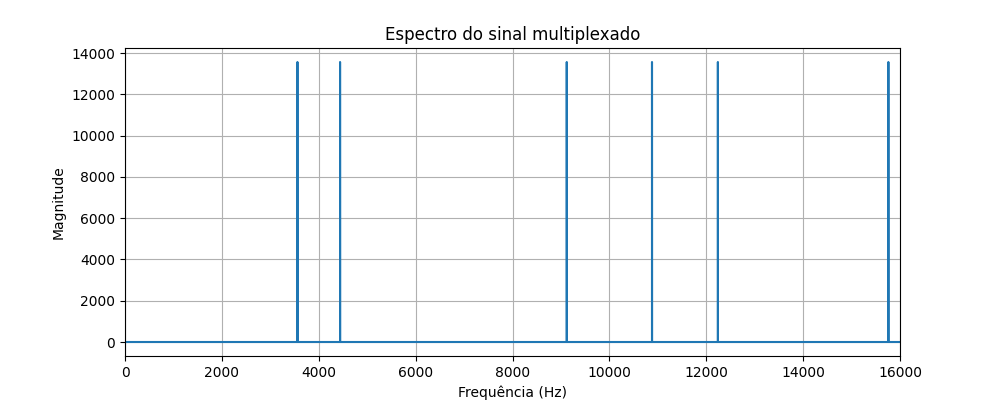
\includegraphics[width=\linewidth]{figura4_espectro.png}
    \captionof{figure}{Espectro do sinal multiplexado mostrando a modulação AM DSB-SC.}
    \label{fig:figura4}
\end{minipage}
\end{center}
\FloatBarrier

Ao juntarmos os três canais, justificam-se os seis picos isolados observados no espectro multiplexado da Figura~\ref{fig:figura4}.

\vspace{1em}

% ============================================================
\section*{Exercício 10}
% ============================================================

\subsection*{Interpretação dos espectrogramas}

As figuras geradas pela função \texttt{compara\_espectro()} representam \textbf{espectrogramas}, isto é, representações tridimensionais do espectro achatadas em duas dimensões. Nessa visualização:

\begin{itemize}
    \item O eixo horizontal (X) representa o \textbf{tempo}, em segundos.
    \item O eixo vertical (Y) representa a \textbf{frequência}, em Hz.
    \item A cor, em forma de mapa de calor, indica a \textbf{amplitude} ou potência do sinal naquela frequência em determinado instante. Tons mais claros, como amarelo e verde, indicam maior energia.
\end{itemize}

\begin{center}
\begin{minipage}{0.8\textwidth}
    \centering
    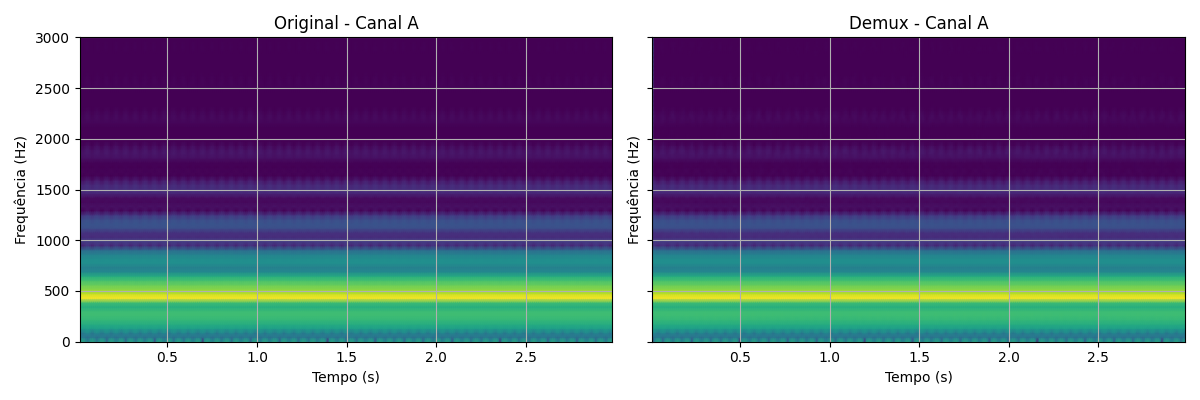
\includegraphics[width=\linewidth]{espectrograma_canal_A.png}
    \captionof{figure}{Comparação de espectrogramas original e demultiplexado do Canal A.}
\end{minipage}
\end{center}
\FloatBarrier

\begin{center}
\begin{minipage}{0.8\textwidth}
    \centering
    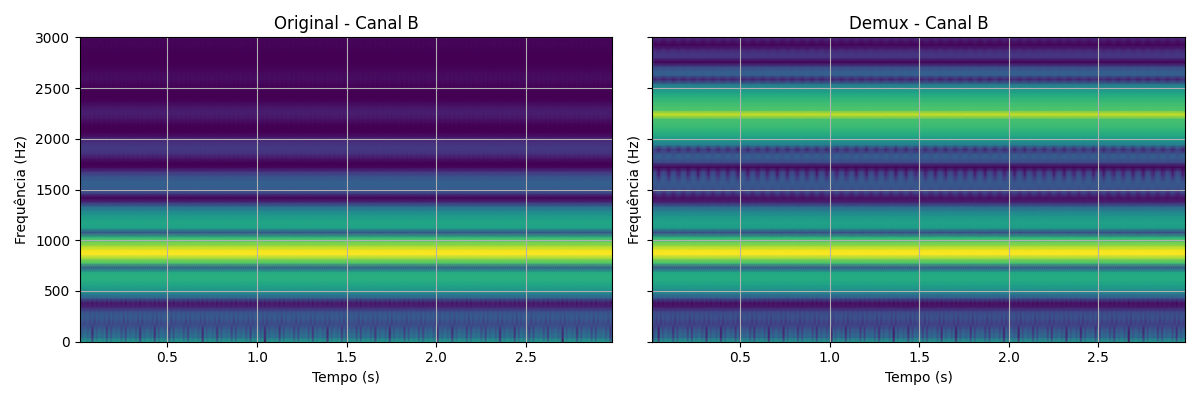
\includegraphics[width=\linewidth]{espectrograma_canal_B.png}
    \captionof{figure}{Comparação de espectrogramas original e demultiplexado do Canal B.}
\end{minipage}
\end{center}
\FloatBarrier

\begin{center}
\begin{minipage}{0.8\textwidth}
    \centering
    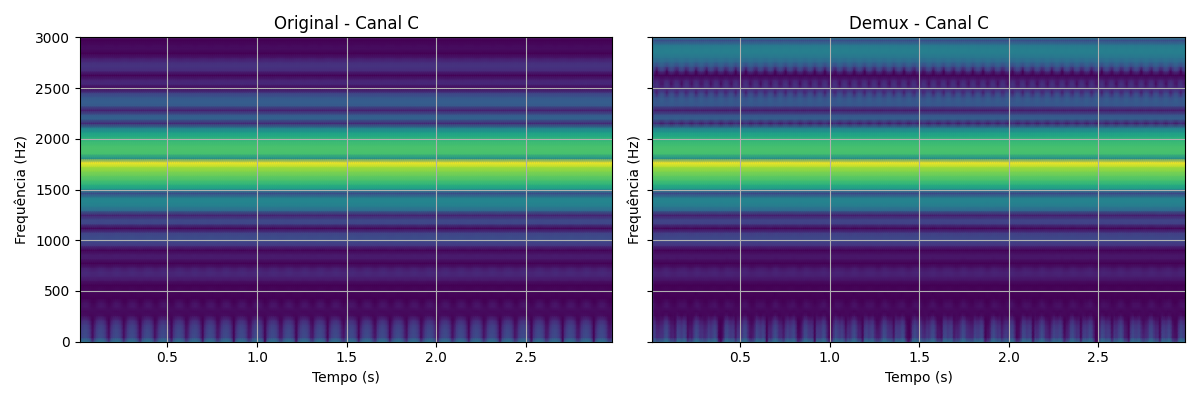
\includegraphics[width=\linewidth]{espectrograma_canal_C.png}
    \captionof{figure}{Comparação de espectrogramas original e demultiplexado do Canal C.}
\end{minipage}
\end{center}
\FloatBarrier

\subsection*{Análise dos resultados}

\textbf{Análise do original:} nos gráficos à esquerda, correspondentes ao sinal original, como os sinais de teste eram ondas senoidais puras, o espectrograma revela uma única linha horizontal luminosa constante durante todo o tempo de gravação. Isso indica que a energia do sinal está concentrada nas frequências de $440$ Hz, $880$ Hz e $1760$ Hz.

\textbf{Análise do demultiplexado:} nos gráficos à direita, correspondentes ao sinal demultiplexado, observa-se que a linha horizontal principal \textbf{reaparece na mesma frequência} correspondente ao sinal original. Isso comprova a eficácia do processo implementado: os filtros passa-banda conseguiram isolar corretamente cada canal na região de alta frequência, a demodulação transladou o sinal de volta para a banda base e o filtro passa-baixa eliminou as frequências indesejadas, resultando na \textbf{recuperação bem-sucedida do sinal da mistura multiplexada}.

\textbf{Avaliação da eficiência:} a recuperação do tom fundamental é altamente eficiente. Contudo, é possível observar pequenos ``fantasmas'' ou ruídos residuais, representados por faixas com coloração levemente diferente do fundo azul escuro. Esses artefatos são causados por imperfeições inerentes aos filtros digitais utilizados. Os filtros \textit{Butterworth} empregados têm ordem fixa igual a 6, o que gera uma atenuação gradual (\textit{roll-off}) em vez de um corte abrupto e ideal. Assim, pequenos fragmentos de outras frequências, ou resíduos de alta frequência ($2f_c$) gerados na demodulação, podem passar pelo filtro e criar esses sutis artefatos visuais. Mesmo assim, o sistema cumpre satisfatoriamente seu papel.

\vspace{1em}

% ============================================================
\section*{Exercício 11 (Bônus)}
% ============================================================

\subsection*{Implementação proposta}

Para a resolução deste bônus, os scripts originais foram unificados e refatorados em uma única classe \texttt{SistemaComunicao}, baseada na biblioteca \texttt{librosa}. O processo foi estruturado para atender aos subitens solicitados.

\subsection*{a) Espectro dos sinais modulados}

O código utiliza \texttt{scipy.fft} para gerar os gráficos no domínio da frequência para as três bandas após a modulação AM DSB-SC, com portadoras em $4000$ Hz, $10000$ Hz e $14000$ Hz.

\begin{center}
\begin{minipage}{0.8\textwidth}
    \centering
    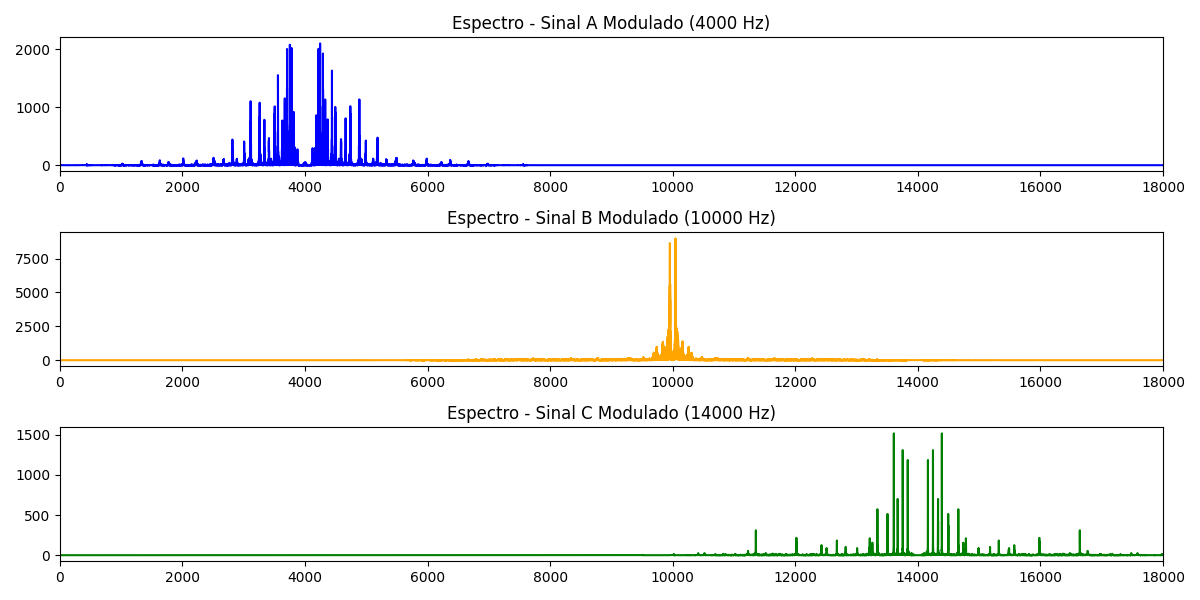
\includegraphics[width=\linewidth]{espectros_individuais.png}
    \captionof{figure}{Espectro dos sinais modulados individualmente.}
\end{minipage}
\end{center}
\FloatBarrier

\subsection*{b) Espectro multiplexado}

Após somar os três sinais modulados, o espectro FDM consolidado foi plotado, exibindo as faixas ocupadas pelos três instrumentos simultaneamente.

\begin{center}
\begin{minipage}{0.8\textwidth}
    \centering
    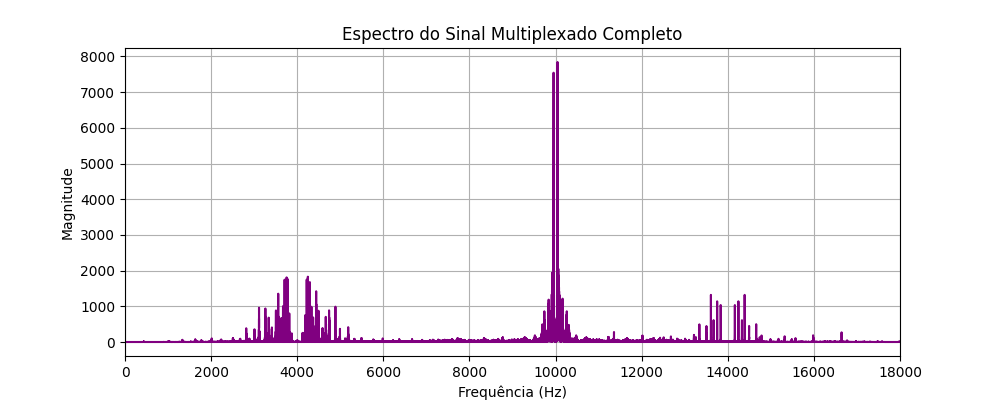
\includegraphics[width=\linewidth]{espectro_multiplexado.png}
    \captionof{figure}{Espectro do sinal multiplexado completo.}
\end{minipage}
\end{center}
\FloatBarrier

\subsection*{c) Salvamento do sinal multiplexado}

O sinal combinado foi salvo localmente usando a biblioteca \texttt{soundfile}, no arquivo \texttt{muxed\_audio.wav}.

\subsection*{d) e e) Demultiplexação e filtragem}

O processo inverso aplica três filtros Passa-Banda do tipo \textit{Butterworth}, de 6ª ordem, nas portadoras alvo para isolar os canais. Em seguida, os sinais são multiplicados novamente por suas respectivas portadoras e passam por filtros Passa-Baixa com frequência de corte em $3000$ Hz, retornando à banda base.

\subsection*{f) Comparação dos áudios}

Ao ouvir e comparar os arquivos \texttt{base\_[Canal].wav}, correspondentes ao sinal ajustado antes do FDM, com os arquivos \texttt{demux\_channel\_[Canal].wav}, notou-se que as características acústicas da voz ou da música foram mantidas inteligíveis e no tom correto.

A limitação a um espectro estreito de $3000$ Hz, necessária para evitar \textit{overlapping} entre os canais, atenuou os agudos e conferiu uma característica semelhante a ``som telefônico''. Apesar disso, essa limitação garantiu a separação dos canais sem interferência cruzada significativa.

\subsection*{g) Código e áudios anexos}

O script final, os arquivos de origem de teste e os resultados em \texttt{.wav} acompanham os anexos desta submissão.

\subsection*{Código-fonte refatorado}

\begin{lstlisting}
import numpy as np
import soundfile as sf
import matplotlib.pyplot as plt
from scipy.fft import fft, fftfreq
from scipy.signal import butter, lfilter
import librosa
import os

class SistemaComunicao:
    def __init__(self):
        # Taxa de amostragem padronizada para todos os audios
        self.fs = 44100 
        # Frequencias das portadoras escolhidas
        self.fc_A = 4000   # Canal A (ex: piano.wav)
        self.fc_B = 10000  # Canal B (ex: bateria.wav)
        self.fc_C = 14000  # Canal C (ex: violao.wav)
        
        # Filtro de corte da banda base. Limitado a 3kHz para evitar 
        # sobreposicao (overlapping) na multiplexacao FDM.
        self.cutoff_baseband = 3000 
        self.order = 6 # Ordem dos filtros Butterworth

    # === Funcoes Auxiliares de Filtros ===
    def lowpass_filter(self, signal, cutoff, fs, order):
        nyq = 0.5 * fs
        b, a = butter(order, cutoff/nyq, btype='low')
        return lfilter(b, a, signal)

    def bandpass_filter(self, signal, lowcut, highcut, fs, order):
        nyq = 0.5 * fs
        b, a = butter(order, [lowcut/nyq, highcut/nyq], btype='band')
        return lfilter(b, a, signal)

    def normalize(self, signal):
        return signal / np.max(np.abs(signal))

    # === Etapa 1: Preparacao do Sinal ===
    def carrega_audios(self):
        print("Carregando arquivos de audio via librosa...")
        a, _ = librosa.load("piano.wav", sr=self.fs, mono=True)
        b, _ = librosa.load("bateria.wav", sr=self.fs, mono=True)
        c, _ = librosa.load("violao.wav", sr=self.fs, mono=True)

        # Truncar todos os audios para o menor tamanho encontrado para podermos somar
        min_len = min(len(a), len(b), len(c))
        a, b, c = a[:min_len], b[:min_len], c[:min_len]

        # Pre-filtragem anti-aliasing (Passa-Baixa em 3000 Hz)
        a = self.lowpass_filter(a, self.cutoff_baseband, self.fs, self.order)
        b = self.lowpass_filter(b, self.cutoff_baseband, self.fs, self.order)
        c = self.lowpass_filter(c, self.cutoff_baseband, self.fs, self.order)

        # Salva os arquivos base normalizados
        sf.write("base_A.wav", self.normalize(a), self.fs)
        sf.write("base_B.wav", self.normalize(b), self.fs)
        sf.write("base_C.wav", self.normalize(c), self.fs)

        return a, b, c, min_len

    # === Etapa 2: Modulacao e Multiplexacao ===
    def multiplexacao(self):
        a, b, c, length = self.carrega_audios()
        t = np.arange(length) / self.fs

        # Modulacao individual de cada sinal (AM DSB-SC)
        a_mod = a * np.cos(2 * np.pi * self.fc_A * t)
        b_mod = b * np.cos(2 * np.pi * self.fc_B * t)
        c_mod = c * np.cos(2 * np.pi * self.fc_C * t)

        # Exibe os espectros individuais
        self.plota_espectros_individuais(a_mod, b_mod, c_mod, length)

        # Soma e normaliza
        muxed = self.normalize(a_mod + b_mod + c_mod)
        sf.write("muxed_audio.wav", muxed, self.fs)
        
        # Exibe o espectro multiplexado
        self.plota_espectro_multiplexado(muxed, length)

        return muxed, length

    # === Etapa 3: Demultiplexacao e Recuperacao ===
    def demultiplexacao(self, muxed, length):
        t = np.arange(length) / self.fs
        carriers = {'A': self.fc_A, 'B': self.fc_B, 'C': self.fc_C}

        print("Iniciando Demultiplexacao...")
        for label, fc in carriers.items():
            band = self.bandpass_filter(muxed, fc - self.cutoff_baseband, fc + self.cutoff_baseband, self.fs, self.order)
            demod = band * np.cos(2 * np.pi * fc * t)
            baseband = self.lowpass_filter(demod, self.cutoff_baseband, self.fs, self.order)
            
            baseband_norm = self.normalize(baseband)
            sf.write(f"demux_channel_{label}.wav", baseband_norm, self.fs)

    # === Funcoes Graficas omitidas no relatorio por simplicidade ===
    # (Elas utilizam scipy.fft para exibir as frequencias na tela)
    def plota_espectros_individuais(self, a, b, c, l): pass
    def plota_espectro_multiplexado(self, muxed, l): pass

if __name__ == "__main__":
    sistema = SistemaComunicao()
    sinal_multiplexado, min_length = sistema.multiplexacao()
    sistema.demultiplexacao(sinal_multiplexado, min_length)
\end{lstlisting}

\end{document}